%%%%%%%%%%%%%%%%%%%%%%%%%%%%%%%%%%%%%%%%%%%%%%%%%%%%%%%%%%%%%%%%%%%%%%%%%%%%%%%%%%%%%%%
%%%%%%%%%%%%%%%%%%%%%%%%%%%%%%%%%%%%%%%%%%%%%%%%%%%%%%%%%%%%%%%%%%%%%%%%%%%%%%%%%%%%%%%
% 
% This top part of the document is called the 'preamble'.  Modify it with caution!
%
% The real document starts below where it says 'The main document starts here'.

\documentclass[12pt]{article}

\usepackage{amssymb,amsmath,amsthm}
\usepackage[top=1in, bottom=1in, left=1.25in, right=1.25in]{geometry}
\usepackage{fancyhdr}
\usepackage{graphicx}
\usepackage{enumerate}
\usepackage{listings}
\usepackage{verbatim}
\usepackage{xcolor}

% Comment the following line to use TeX's default font of Computer Modern.
\usepackage{times,txfonts}


\definecolor{codegreen}{rgb}{0,0.6,0}
\definecolor{codegray}{rgb}{0.5,0.5,0.5}
\definecolor{codepurple}{rgb}{0.58,0,0.82}
\definecolor{backcolour}{rgb}{0.95,0.95,0.92}

\lstdefinestyle{mystyle}{
    backgroundcolor=\color{backcolour},   
    commentstyle=\color{codegreen},
    keywordstyle=\color{magenta},
    numberstyle=\tiny\color{codegray},
    stringstyle=\color{codepurple},
    basicstyle=\ttfamily\footnotesize,
    breakatwhitespace=false,         
    breaklines=true,                 
    captionpos=b,                    
    keepspaces=true,                 
    numbers=left,                    
    numbersep=5pt,                  
    showspaces=false,                
    showstringspaces=false,
    showtabs=false,                  
    tabsize=2
}

\lstset{style=mystyle}

\newtheoremstyle{homework}% name of the style to be used
  {18pt}% measure of space to leave above the theorem. E.g.: 3pt
  {12pt}% measure of space to leave below the theorem. E.g.: 3pt
  {}% name of font to use in the body of the theorem
  {}% measure of space to indent
  {\bfseries}% name of head font
  {:}% punctuation between head and body
  {2ex}% space after theorem head; " " = normal interword space
  {}% Manually specify head
\theoremstyle{homework} 

% Set up an Exercise environment and a Solution label.
\newtheorem*{exercisecore}{\@currentlabel}
\newenvironment{exercise}[1]
{\def\@currentlabel{#1}\exercisecore}
{\endexercisecore}

\newcommand{\localhead}[1]{\par\smallskip\noindent\textbf{#1}\nobreak\\}%
\newcommand\solution{\localhead{Solution:}}



% \newcommand{includematlab}[1]{\verbatiminput{#1}}

%%%%%%%%%%%%%%%%%%%%%%%%%%%%%%%%%%%%%%%%%%%%%%%%%%%%%%%%%%%%%%%%%%%%%%%%
%
% Stuff for getting the name/document date/title across the header
\makeatletter
\RequirePackage{fancyhdr}
\pagestyle{fancy}
\fancyfoot[C]{\ifnum \value{page} > 1\relax\thepage\fi}
\fancyhead[L]{\ifx\@doclabel\@empty\else\@doclabel\fi}
\fancyhead[C]{\ifx\@docdate\@empty\else\@docdate\fi}
\fancyhead[R]{\ifx\@docauthor\@empty\else\@docauthor\fi}
\headheight 15pt

\def\doclabel#1{\gdef\@doclabel{#1}}
\doclabel{Use {\tt\textbackslash doclabel\{MY LABEL\}}.}
\def\docdate#1{\gdef\@docdate{#1}}
\docdate{Use {\tt\textbackslash docdate\{MY DATE\}}.}
\def\docauthor#1{\gdef\@docauthor{#1}}
\docauthor{Use {\tt\textbackslash docauthor\{MY NAME\}}.}
\makeatother

%% General formatting parameters
\parindent 0pt
\parskip 12pt plus 1pt

% Shortcuts for blackboard bold number sets (reals, integers, etc.)
\newcommand{\Reals}{\ensuremath{\mathbb R}}
\newcommand{\Nats}{\ensuremath{\mathbb N}}
\newcommand{\Ints}{\ensuremath{\mathbb Z}}
\newcommand{\Rats}{\ensuremath{\mathbb Q}}
\newcommand{\Cplx}{\ensuremath{\mathbb C}}
%% Some equivalents that some people may prefer.
\let\RR\Reals
\let\NN\Nats
\let\II\Ints
\let\CC\Cplx

%%%%%%%%%%%%%%%%%%%%%%%%%%%%%%%%%%%%%%%%%%%%%%%%%%%%%%%%%%%%%%%%%%%%%%%%%%%%%%%%%%%%%%%
%%%%%%%%%%%%%%%%%%%%%%%%%%%%%%%%%%%%%%%%%%%%%%%%%%%%%%%%%%%%%%%%%%%%%%%%%%%%%%%%%%%%%%%
% 
% The main document start here.

% The following commands set up the material that appears in the header.
\doclabel{Math 426: Homework 3}
\docauthor{Andrew Player}
\docdate{September 16, 2020}

\newcommand{\vv}{\mathbf{v}}
\begin{document}

\begin{exercise}{DM 1}
Write down the $4^{\rm th}$ order Taylor
polynomial of $\sqrt{x}$ centered at $x=1$.  Let
$P(x)$ denote this polynomial. If $1\le x \le 2$,
what can you say about the size of $|\sqrt{x}-P(x)|$?
Hint: Use the remainder term!
\end{exercise}
\solution
\begin{equation}
1+\frac{x-1}{2}-\frac{1}{8}(x-1)^2+\frac{1}{16}(x-1)^3
\end{equation}
The size of the difference gets larger from 1 to 2.

\begin{exercise}{Chapter 4: 2 (c)}

For full credit you must write your own version of Newton's method.
Your function should have the signature

\begin{verbatim} 
function [r,hist] = hw3newton(f,fp,x1,ftol,xtol,Nmax)

end
\end{verbatim}

The input values are
\begin{itemize}
\item \texttt{f}, the function to find a root of.
\item \texttt{fp}, the derivative function of \texttt{f}.
\item \texttt{x1}, the first iteration value.
\item \texttt{ftol}, the tolerance for stopping based of the value of \texttt{f}
\item \texttt{xtol}, the tolerance for stopping based on changes in \texttt{x}
\item \texttt{Nmax}, the maximum number of iterations
\end{itemize}

Your function should exit with an error if more than \texttt{Nmax} iterations
are used.  It should return whenever $|f(x)|<f_{\text{tol}}$ or $|x_n-x_{n-1}|<x_{\text{tol}}$.

The return values should be \texttt{r}, the estimate of the root's position,
and \texttt{hist}, a list of all estimates starting with \texttt{x1} and ending with the final estimate \texttt{r}.

Test that your function works by finding three different ways to call it
so that iteration stops for each of the three possible reasons.

To answer the problem in the textbook, you will want to call your functin with 
$x_{\rm tol}=0$ to ensure that only the $f_{\rm tol}$ condition is used
to stop the iteration.
\end{exercise}
\begin{verbatim}

\end{verbatim}
Code:
\begin{lstlisting}[language=Matlab]
function [r,hist] = hw3newton(f, fp, x1, ftol, xtol, Nmax)
    
  %X_{k}
  current_value = x1;
  %X_{k-1}
  last_value = x1;
  
  iterations = 0;
  hist = [current_value];
  
  while(true)
      if(iterations > Nmax)
          error("Iteration Count Exceeded")
      end
      
      % Check if f(X_k) is sufficiently small
      if(abs(f(last_value)) < ftol)
          r = last_value;
          return
      end
      
      % Do the iteration
      last_value = current_value;
      current_value = current_value-f(current_value)/fp(current_value);
      iterations = iterations + 1;
      
      % Check if |X_(k) - X_(k-1)| is sufficiently small
      if(abs(current_value - last_value) < xtol)
          r = current_value;
          return
      end

      hist = [hist ;last_value];
  end
end
\end{lstlisting}
Output:
\begin{lstlisting}[language=Matlab]
>> func = @(x) ((5-x)*exp(x)-5);
>> funcp = @(x) (-exp(x)*(x-4));
>> xtol = 0;
>> ftol = 1e-8;
>> x1 = 5;
>> Nmax = 25;
>> [r,hist] = hw3newton(func, funcp, x1, ftol,xtol, Nmax);
>> r

r =

  4.965114231746430

>> hist

hist =

  5.000000000000000
  4.966310265004573
  4.965115686301458
  4.965114231746430
\end{lstlisting}
\begin{verbatim}
It should take 1 more iterations to get to 1e-16.
\end{verbatim}

\begin{exercise}{Chapter 4: 6 (a,b)}
Also, use your \texttt{hw3newton} function from the previous problem
to compute the location of the minimum, and generate a plot that indicates that your computation succeeded.
\end{exercise}
\solution 
Part(a):
The function has a minimum where h'(x) = 0, so f(x) = h'(x). Therefore, the netwons method formula
for this function is:
\begin{equation}
x_{k} = x_{k-1} - \frac{f(x_{k-1})}{f'(x_{k-1})} = x_{k-1} - \frac{x_{k-1}^3-3}{3x_{k-1}^2}
\end{equation}
\solution
Part(b): 
\begin{equation}
x_{1} = 1 - \frac{(1)^3-3}{3(1)^2} = \frac{5}{3}
\end{equation}
Compute:
\begin{lstlisting}[language=Matlab]
>> func = @(x) (x.^4)/4-3*x;
>> h = @(x) x.^3 - 3;
>> hp = @(x) (3*x.^2);
>> [r,hist] = newton(h, hp, x1, ftol, xtol, Nmax);
>> r

r =

    1.442249570307408
\end{lstlisting}
This looks good compared to the plots:
\newline
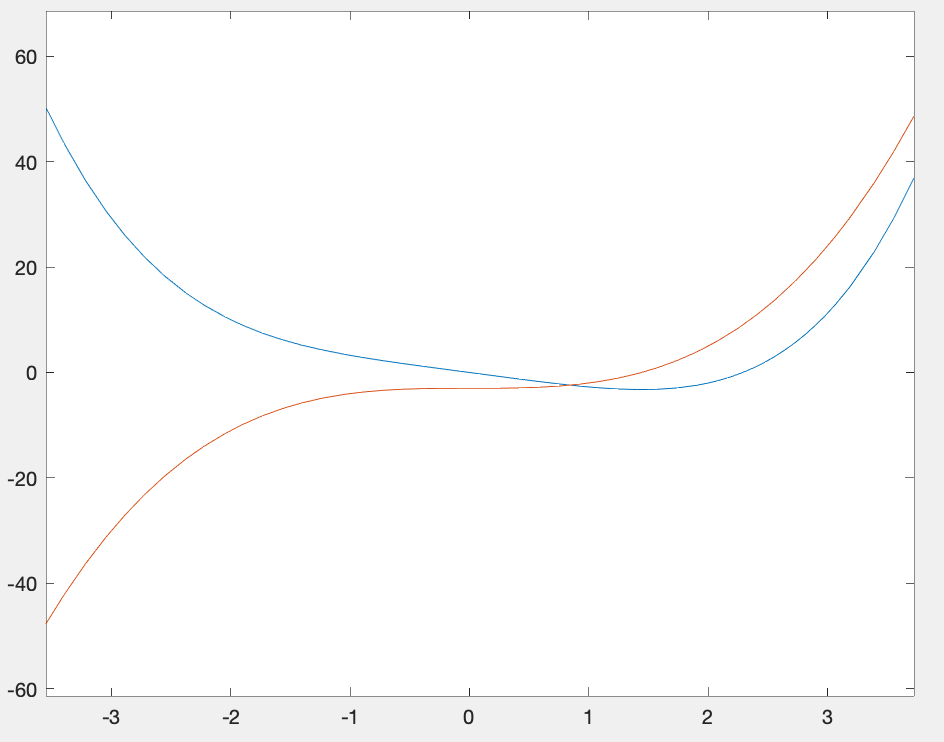
\includegraphics[scale=0.5]{original.png}
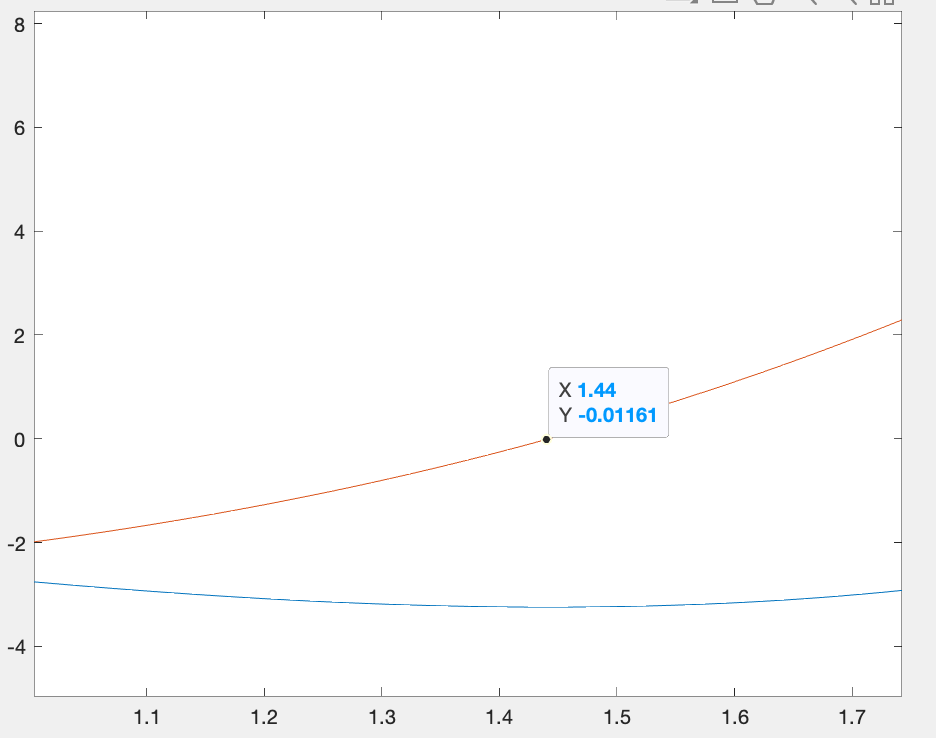
\includegraphics[scale=0.5]{zoomed.png}

\begin{exercise}{Chapter 4: 7}
\end{exercise}
\begin{equation}
x_1 = 4 - \frac{1}{f'(4)} = 3 
\end{equation}
\begin{equation}
\frac{1}{f'(4)} = 1
\end{equation}
\begin{equation}
f'(4) = 1
\end{equation}

\begin{exercise}{Chapter 4: 10}
The function is discontinous at x=2, therefore the bisection
will simply blow up to infinity rather than go towards the root.
\end{exercise}

\end{document}